\lhead[\thepage]{CAPÍTULO \thechapter. \rightmark}
\rhead[CAPÍTULO \thechapter. \leftmark]{\thepage}
%======================================================================
\chapter{Teoría de conjuntos}
\label{TC}
\markboth{Teoría de conjuntos}{Teoría de conjuntos}
%======================================================================


%----------------------------------------------------------------------
\section{Cuantificadores lógicos}
\label{TC0}
%----------------------------------------------------------------------

Hasta el momento en la sección (\ref{LM}) se han revisado proposiciones, las cuales son verdaderas o falsas y no cambia esta condición a menos que se aplique el operador lógico de la negación. Hay un tipo de proposiciones, como por ejemplo las inecuaciones, que para algunos valores de la variable la proposición es verdadera y para otros es falsa.
\begin{equation}
x > \pi
\label{xpi}
\end{equation}
De la ecuación anterior (\ref{xpi}) se puede ver que cuando la variable $x$ toma valores mayores que $\pi$\footnote{$\pi$ es un número con infinitos decimales e irracional, es decir, no se puede representar como una fracción. $\pi=3,141592653...$} esta proposición es verdadera, pero para cualquier otro caso ($x$ menores que $\pi$) es una proposición falsa. Ahora estas proposiciones pueden tener $n$ variables, entonces la proposición pasa a ser una \textit{función proposicional}.

\begin{mydef}
\textbf{Función proposicional}. Es una expresión que contiene una o más variables, y pasa a ser una proposición si se asigna valores específicos a las variables.
\end{mydef}
\begin{eqnarray}
p(x_{1},x_{2},x_{3},...,x_{n})\label{fp0}\\
p(x): \underbrace{x}_\text{sujeto} \underbrace{tiene\hspace{3px} la\hspace{3px} propiedad\hspace{3px} p}_\text{predicado}
\label{fp1}
\end{eqnarray}
Para el conjunto de valores que hace verdadera las funciones proposicionales (\ref{fp0}) y (\ref{fp1}) se llama \textit{conjunto de validez}

\begin{mydef}\label{def:def444}
\textbf{Conjunto de validez}. Se llama conjunto de validez de una función proposicional al conjunto de todos los valores de las variables $x_{1}, x_{2},...,x_{n}$ que la convierten en una proposición verdadera 
\end{mydef}

\begin{myexample}
Encontrar el conjunto de validez ($V_{p}$) de las siguientes proposiciones:
\end{myexample}
\begin{eqnarray}
p(x)&:& \hspace{6px} x-3=5\nonumber\\
p(x)&:& \hspace{6px} x=5+3\nonumber\\
p(x)&:& \hspace{6px} x=8
\end{eqnarray}
Conjunto de validez es 8, o dicho de otra manera $x\in \{8\}$.\\

\begin{eqnarray}
p(x)&:& \hspace{6px} x^{2}=4\nonumber\\
p(x)&:& \hspace{6px} \sqrt{x^{2}}=\sqrt{4}\nonumber\\
p(x)&:& \hspace{6px} x=\pm 2
\end{eqnarray}
El conjunto de validez son los números $2$ y $-2$, o dicho de otra manera $x\in\{-2,2\}$.\\

Notar que $p(x)$ no es una proposición como tal, pero cuando $x=a$ y pasa a ser $p(a)$ si lo es. Ahora otra forma de aludir a un conjunto de validez es usando los cuantificadores. 

\begin{mydef}
\textbf{Cuantificador universal}. Dado un enunciado abierto $p(x)$ con una variable x, el enunciado $\forall x, p(x)$ se lee ``para todo $x$, $p(x)$'' y es verdadero cuando el conjunto de verdad es el universo completo. Se simboliza con $\forall$ y se llama \textbf{cuantificador universal}.
\end{mydef}

\begin{mydef}
\textbf{Cuantificado existencial}. Se llama \textbf{cuantificador existencial} al símbolo $\exists$ y se lee ``existe x tal que $p(x)$'' y es verdadero cuando el conjunto de verdad para la proposición $p(x)$ no es vacío.
\end{mydef}

\begin{myexample}
Si el conjunto universo es $\mathbb{N}$\footnote{Conjunto de números enteros que comienzan en el cero. $\mathbb{N}=\{0,1,2,3,...\}$.}, $p(x):x+4>3$ y $q(x):x+2<8$, entonces:
\end{myexample}

$V_{p}=\mathbb{N}$, es decir, ``para todo $x$, $x$ en $\mathbb{N}$, $p(x)$ es verdadera''. En términos de cuantificadores se escribe $\forall x,x\in\mathbb{N},p(x)$.\\

$V_{q}=\{1,2,3,4,5\}$, es decir, ``Existe (o existe algún) $x$, $x$ en $\mathbb{N}$, tal que $q(x)$ es verdadera''. En términos de cuantificadores se escribe $\exists x,x\in\mathbb{N},q(x)$.

\begin{itemize}
\item Algunas observaciones.
	\subitem - Sea el conjunto universo denotado por $\mathcal{U}$.
	
	\subitem - Si el conjunto de validez tiene un solo elemento, el cuantificador $\exists$ pasa a $\exists!$. Se escribe ``$\exists! x, x\in\mathcal{U},p(x)$'' y se lee ``existe un único $x\in\mathcal{U}$ tal que $p(x)$ es verdadero''.
	
	\subitem - La negación de la proposición  ``Para todo $x$ en $\mathcal{U}$, $p(x)$ es verdadera'' es ``No es verdad que para todo $x$ en $\mathcal{U}$, $p(x)$ es verdadera'' o también ``Existe un $x$ en $\mathcal{U}$ tal que la proposición $\sim p(x)$ es verdadera''. En términos de cuantificadores se escribe:
	\begin{equation}
	\sim(\forall x,x\in\mathcal{U},p(x))\Leftrightarrow(\exists x,x\in\mathcal{U},\sim p(x))
	\end{equation}
	
	\subitem - La negación de la proposición ``Existe un $x$ en $\mathcal{U}$ tal que $p(x)$ es verdadera'' es ``No es verdad que existe un $x$  en $\mathcal{U}$ tal que la proposición $p(x)$ es verdadera'' o ``Para todo $x$ en $\mathcal{U}$, la proposición $p(x)$ es falsa''. En términos de cuantificadores se escribe:
	\begin{equation}
	\sim(\exists x,x\in\mathcal{U},p(x))\Leftrightarrow(\forall x,x\in\mathcal{U},\sim p(x))
	\end{equation}
\end{itemize}

	\subitem - La negación de la proposición ``Existe un único $x$ en $\mathcal{U}$ tal que $p(x)$ es verdadera'' es ``no existe ningún $x$ en $\mathcal{U}$ tal que $p(x)$ es verdadera o existen al menos dos elementos en $\mathcal{U}$, $x$ e $y$, tales que $p(x)$ y $p(y)$ son verdaderas''. En términos de cuantificadores se escribe:
	\begin{equation}
	\sim(\exists!x,x\in\mathcal{U},p(x))\Leftrightarrow(\forall x,x\in\mathcal{U},\sim p(x))\vee(\exists x,x\in\mathcal{U},\exists y,y\in\mathcal{U},p(x),p(y))
	\end{equation}
	
\begin{myexample}
Encontrar el conjunto de validez y escribir la proposición con cuantificadores
\end{myexample}
Si $\mathcal{U}=\mathbb{N}$, entonces $p(x):x+2=9$ es verdadera sólo para $x=7$, esto significa que el conjunto de validez es $V_{p}=\{7\}$ y con cuantificadores se escribe:
\begin{equation}
\exists!x,x\in\mathbb{N}\hspace{3px}tal\hspace{3px}que\hspace{3px}x+2=9
\end{equation}

\begin{myexample}
Negar la proposición  $(\forall x,x\in \mathbb{Z},x+5\leq 10)$: \\

La negación de $(\forall x,x\in \mathbb{Z},x+5\leq 10)$ es $(\exists x,x\in \mathbb{Z},x+5>10)$.\footnote{$\mathbb{Z}$ son todos los números enteros. $\mathbb{Z}=0,\pm 1,\pm 2, \pm 3,...$}
\end{myexample}

\begin{myexample}
Negar la proposición  $(\exists x,$ $x\in\mathbb{R}, x=20)$: \\

La negación de $(\exists x,$ $x\in\mathbb{R}, x=20)$ es  $(\forall x,$ $x\in\mathbb{R}, x\neq 20)$
\end{myexample}
\newpage
\section{Conjuntos y elementos}
\label{CyE}

Es natural querer agrupar ciertos números u objetos bajo una misma característica o condición para obtener algún tipo de información. Bajo esta premisa nacen los \textit{conjuntos} y quienes los conforman se llaman \textit{elementos} del conjunto. Cuando se dice que un elemento pertenece a un conjunto se denota con el símbolo ya utilizado $\in$ que se lee ``pertenece a'' y para el caso contrario, en que no pertenezca se usa el $\notin$ que se lee ``no pertenece a''.

\begin{mydef}
\textbf{Conjunto}. Un conjunto es una colección bien definida de objetos, llamados sus elementos. Los conjuntos se simbolizan con letras mayúsculas $A$, $B$, $C,...$. Los objetos que componen el conjunto se denominan elementos o miembros y se denotan con letras minúsculas $a$, $b$, $c$,$...$
\end{mydef}

Un conjunto es una entidad con naturaleza diferente a los elementos que lo componen. Entonces se debe aclarar que siendo $A$ un conjunto, se cumple que $A=\{a\}\neq a$ y $\{a\}$ no es un elemento de $A$.\\

 Algunas observaciones y definiciones de los conjuntos:
\begin{itemize}

	\item El conjunto que no contiene elementos se llama \textit{conjunto vacío} y se denota por $\emptyset$ o $A=\{\}$.
	\item El conjunto de un solo elemento se llama conjunto unitario.
	\item Si $x$ es un elemento del conjunto $A$ se escribe $x\in A$ y se lee ``$x$ pertenece a $A$''. La negación de la proposición anterior es $x\notin A$ y se lee ``$x$ no pertenece a $A$''.
	\item Un conjunto es bien definido cuando dado un objeto cualquiera, se puede definir si pertenece o no al conjunto $A$.
	\item Un conjunto se puede ser definido de dos maneras:\\
		\subitem - Nombrando sus elementos. Este tipo de conjuntos se definen por \textit{extensión}.\\
		\subitem - Nombrando una propiedad que caracteriza a sus elementos. Este tipo de conjuntos se definen por \textit{comprensión}.
\end{itemize}

\begin{mydef}
\textbf{Conjunto de extensión y comprensión}. Para escribir un conjunto por extensión, se enumeran todos sus elementos separándolos con comas y luego se encierran entre llaves $\{...\}$.\\
Para escribir un conjunto por comprensión se elige un elemento arbitrario x y se señala que cumple la propiedad p(x). Finalmente, se encierra toda la expresión entre llaves:\\
\begin{equation*}
A=\{x|x\hspace{3px}p(x)\}
\end{equation*}
que se lee ``A es el conjunto de todos los elementos x tales que los x cumplen la propiedad p(x)''. El símbolo $|$ se lee ``tal que''.
\end{mydef}

\begin{myexample}\label{ejemplosNR}
Algunos conjuntos de números importantes.
\end{myexample}
\noindent $\mathbb{N}=\{1,2,3,...\}$ \textit{Conjunto de los números naturales.}\\
$\mathbb{Z}=\{0,\pm 1,\pm 2,\pm 3,...\}$ \textit{Conjunto de los números enteros.}\\
$\mathbb{R}=\{x,x$ \textit{es un número decimal}$\}$ \textit{Conjunto de los números reales.}\\
$\mathbb{Q}=\{\dfrac{a}{b}:a\in\mathbb{Z},b\in\mathbb{Z},b\neq 0\}$ \textit{Conjunto de los números racionales}\\
$\mathbb{I}=\{x:x\in\mathbb{R}\wedge x\notin\mathbb{Q}\}$ \textit{Conjunto de los números irracionales.}

Notar que los conjuntos $\mathbb{N}$ y $\mathbb{Z}$ están definidos por extensión, mientras que los conjuntos $\mathbb{R}$, $\mathbb{Q}$ y $\mathbb{I}$ por comprensión. Además, los tres puntos suspensivos muestran que el conjunto seguirá el mismo patrón para todos los elementos restantes.\\

\begin{mydef}
\textbf{Conjuntos iguales}. Sea A y B dos conjuntos, si ambos conjuntos contienen los mismos elementos, estos conjuntos se llaman \textbf{conjuntos iguales} y se escriben de la siguiente manera:
\begin{equation*}
A=B
\end{equation*}
\label{conjutosiguales}
\end{mydef}
Con la definición (\ref{conjutosiguales}) se desprende que conjuntos $\{a,b,c,d\}$, $\{b,c,a,d\}$ y $\{a,a,b,c,c,d\}$ son iguales, es decir, no importa el orden ni la repetición de los elementos. Lo que interesa es cuantos tipos de elementos diferentes hay dentro del conjunto.

\begin{mydef}
\textbf{Conjuntos finitos}. Si un conjunto contiene elementos igual a un número natural, se llama un conjunto finito.
\end{mydef}

\begin{mydef}
\textbf{Conjuntos infinitos}. Si un conjunto contiene un número ilimitado de elementos se llaman conjuntos infinitos.
\end{mydef}

\begin{myexample}
Defina si los siguientes conjuntos son finitos o infinitos.\\

\noindent Sea $A=\{5,6,3,9\}$ un conjunto. $A$ se define como un conjunto finito.\\

\noindent Sea $B=\{x|x$ \textit{es un número entero positivo}$\}$ un conjunto. $B$ se define como un conjunto infinito.
\end{myexample}


Hasta el momento solo se menciona número de elementos de un conjunto, pero desde ahora en adelante se hablará \textit{cardinalidad} de un conjunto dado.\\

\begin{mydef}\label{cardinalidad}
\textbf{Cardinalidad}. El número de elementos de un conjunto finito se llama cardinalidad. La cardinalidad de un conjunto finito A se denota por:\\
\begin{equation*}
Card(A) \hspace{3px} o \hspace{3px} |A| \hspace{3px} o \hspace{3px} \#A 
\end{equation*}
\end{mydef}

\begin{myexample}
Escriba la cardinalidad de los siguientes conjuntos:\\

\noindent Sea $A=\{h,i,j,k,l,n\}$ un conjunto. La cardinalidad de $A$ es $6$, o escrito de otra manera es $Card(A)=6$\\

\noindent Sea $A=\{a,b,a,a,b\}$ un conjunto. La cardinalidad de $A$ es $2$, o escrito de otra manera $Card(A)=2$.\\

\noindent Sea $A=\{-5,0,5\}$ y $B=\{1,3,7\}$ dos conjuntos ¿Cuál es la suma de las cardinalidades?. La respuesta es $|A|+|B|=6$.
\end{myexample}


\begin{mydef}
\textbf{Conjuntos equipotentes}. Dos conjuntos X e Y se dicen ser equipotentes si tienen exactamente el mismo número de elementos.
\end{mydef}

\begin{mydef}\label{conjuntoU}
\textbf{Conjunto universal. }En cualquier aplicación de la teoría de conjuntos, los elementos de todos los conjuntos pertenecen usualmente a un gran conjunto fijo llamado conjunto universal. Este se denota por $\mathcal{U}$
\end{mydef}

\begin{mydef}
\textbf{Subconjunto}. Si cada elemento de un conjunto de A es también un elemento de un conjunto B, entonces se dice que A es un subconjunto de B. Se dice también que A está contenido en B o que B contiene a A. La relación de subconjunto viene dada por:\\
\begin{equation*}
A\subset B \hspace{3px} o \hspace{3px} B\supset A
\end{equation*} 
En términos de cuantificadores se escribe $A\subset B\Leftrightarrow (x\in A\Rightarrow x\in B)$.
\end{mydef}

\begin{myexample}
Muestra de conjuntos equipotentes, conjunto universo y subconjunto.\\

\noindent Sea $A=\{a,e,i,o,u\}$ y $B=\{lunes$, $martes$, $mi\acute{e}rcoles$, $jueves$, $viernes\}$ dos conjuntos finitos. $A$ y $B$ son conjuntos equipotentes, ya que $|A|=|B|=5$.\\

\noindent Si se hace una consulta a comunidades humanas, entonces un ejemplo de un conjunto universal sería los habitantes de algún país en específico.\\

\noindent Sea $A=\{1,2,a,b\}$ y $B=\{1,b\}$ don conjuntos finitos. Como todos los elementos de $B$ están contenidos en el conjunto $A$, entonces se puede decir que $B\subset A$.
\end{myexample}


\begin{mydef}
\textbf{Conjunto potencia}. El Conjunto de todos los subconjuntos de un conjunto dado A, se llama conjunto de partes o conjunto potencia y se denota como $\mathcal{P}(A)$. Se escribe de la siguiente manera:
\begin{equation*}
\mathcal{P}(A)=\{X: X\subset A\}
\end{equation*}
\end{mydef}

El conjunto de partes $\mathcal{P}(A)$ nunca es vacío, puesto que el conjunto vacío y el mismo conjunto $A$ son elementos de $\mathcal{P}(A)$. Además, si $A$ tiene $n$ elementos, entonces $\mathcal{P}(A)$ contiene $2^{n}$ elementos.

\begin{myexample}
Sea $A=\{0,1,2\}$ un conjunto finito, entonces el conjunto potencia de $A$ es:
\end{myexample}
\begin{equation*}
\mathcal{P}(A)=\{\emptyset,\{0\},\{1\},\{2\},\{0,1\},\{0,2\},\{1,2\},A\}
\end{equation*} 

\begin{myexample}
Sea $A=\{0,1\}$ un conjunto finito. Calcule el conjunto potencia de $A$.\\
\begin{eqnarray*}
\mathcal{P}(A)=\{\emptyset,A,\{0\},\{1\}\}
\end{eqnarray*}
Debe notar que $\{1\}\in \mathcal{P}(A)$ y $\{\{1\}\}\subset \mathcal{P}(A)$.
\end{myexample}
 

\begin{itemize}
\item Algunas propiedades de los conjuntos $A$, $B$ y $C$.\\
	\subitem - $\emptyset \subset A$
	\subitem - $A\subset A$
	\subitem - $\emptyset\subset A$
	\subitem - $[(A\subset B)\wedge(B\subset C)]\Rightarrow A\subset C$
	\subitem - $[(A\subset B)\wedge(B\subset A)]\Leftrightarrow A=B$
\end{itemize} 

\section{Operaciones con conjuntos}
\label{opc}
Aquí es donde se relaciona los conceptos antes vistos de cuantificadores lógicos (sección \ref{TC0}) y la teoría de conjuntos (sección \ref{CyE}). Además, se debe recordar la definición (\ref{conjuntoU}) que en palabras mas simples es el que contiene todos los elementos de interés para el estudio.\\

Al momento de plasmar explícitamente los conjuntos vimos que están los cuantificadores que ayudan, pero otra herramienta que se ocupa es el diagrama de Venn\footnote{Diagrama que recibe el nombre por el matemático y lógico británico John Venn (1834-1923).} que sirve para mostrar gráficamente los conjuntos, sus intersecciones y uniones.\\

El diagrama de Venn muestra de forma gráfica la relación entre conjuntos, donde el caso de dos o tres conjuntos se puede representar con círculos. El diagrama muestra todas las relaciones lógicas posibles con la superposición entre los círculos que representa cada conjunto.\\
\begin{center}
	\begin{figure}[ht!]
	\centering
    		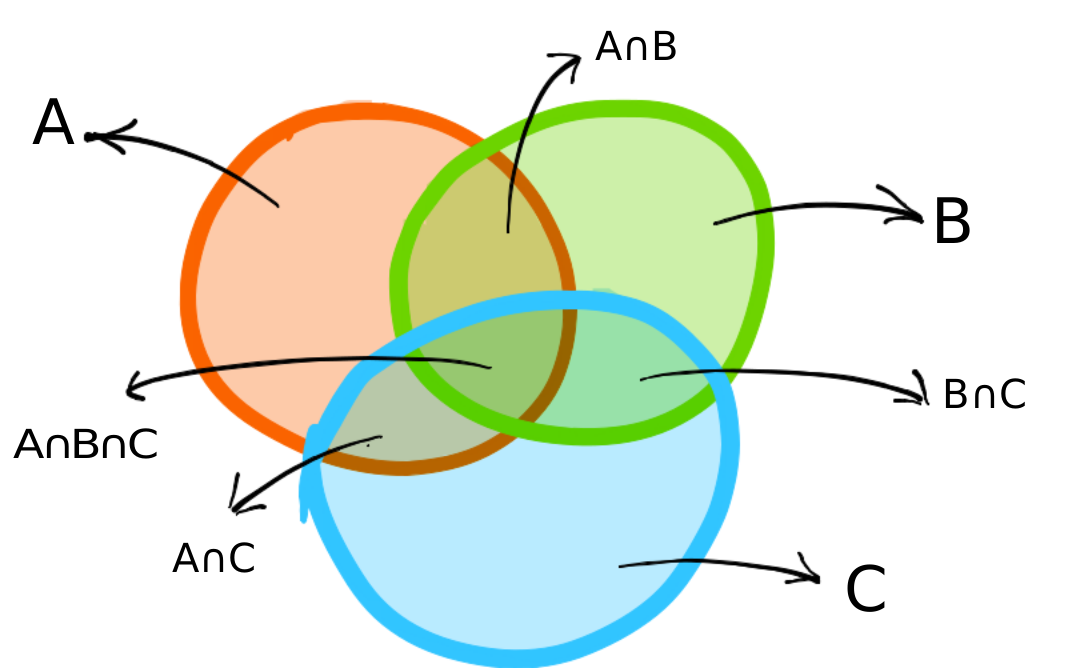
\includegraphics[scale=0.35]{FiguresBM/DV0.png}
    		\caption[Representación del diagrama de Venn para tres conjuntos]{Representación del diagrama de Venn para tres conjuntos. El círculo naranjo representa el conjunto $A$, el círculo verde representa el conjunto $B$ y el circulo celeste representa el conjunto $C$. Las secciones que se superponen dos círculos muestran la intersección de dos conjuntos y la superposición central es la intersección de los tres conjuntos.}
	\end{figure}
\end{center}

\subsection{Diferencia de conjuntos}
La diferencia entre dos conjuntos $A$ y $B$ es el conjunto de los elementos que pertenecen a $A$ y no pertenecen a $B$. La diferencia entre $A$ y $B$ se denota como $A-B$ o $A|B$. Escrito con cuantificadores queda de la siguiente manera: \\

\begin{equation}
A-B =\{x\in\mathcal{U}:x\in A\wedge x\notin B\}=\{x|x\in A\wedge x\notin B\}
\label{dif0}
\end{equation}
\begin{myexample}
Dado dos conjuntos finitos $A=\{a,b,c,d,e,f\}$ y $B=\{c,d,e,f,g,h\}$ determinar la diferencia $A-B$
\end{myexample}
Como se vio en la definición el conjunto resultante son los elementos que están en el conjunto $A$ pero no están en el conjunto $B$
\begin{equation*}
A-B=\{a,b\}
\end{equation*}

\begin{center}
	\begin{figure}[ht!]
	\centering
    		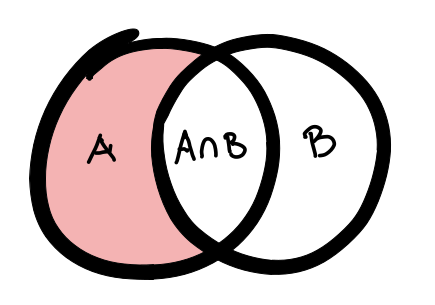
\includegraphics[scale=0.35]{FiguresBM/diferenciac.png}
    		\caption[Representación de diferencia de dos conjuntos]{Representación de diferencia de dos conjuntos usando el diagrama de Venn. Zona marcada con rojo marca $A-B$.}
	\end{figure}
\end{center}

se sacan los elementos que puedan estar en la intersección de ambos conjuntos y exclusivamente en el conjunto B.

\subsection{Complemento de un conjunto}
Dado el conjunto $A$, $\mathcal{U}-A$ se llama complemento de $A$ con respecto a $\mathcal{U}$ y se denota como $A^{c}$, $A'$ o $-A$. Entonces, en términos de cuantificadores lógicos el complemento se escribe de la siguiente manera:
\begin{equation}
A^{c}=\{x\in\mathcal{U}:x\notin A\}
\end{equation}
De la definición anterior se verifica que $\forall x\in\mathcal{U}$  una y solo una de la siguientes proposiciones:
\begin{equation*}
i)\hspace{2px} x\in A \hspace{20px} ii)\hspace{2px} x\in A^{c}
\end{equation*}

\begin{center}
	\begin{figure}[ht!]
	\centering
    		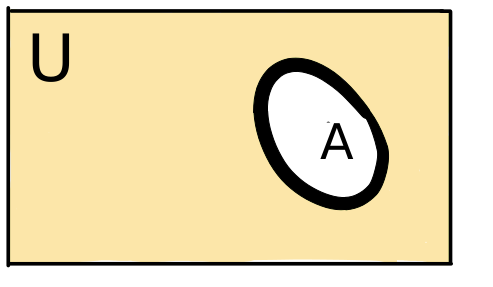
\includegraphics[scale=0.38]{FiguresBM/complemento.png}
    		\caption[Representación del complemento del conjunto $A$]{Representación del complemento del conjunto $A$. La zona oscurecida muestra el conjunto complemento, donde $\mathcal{U}$ es el conjunto universal.}
	\end{figure}
\end{center}

\subsection{Intersección de conjuntos }
La intersección de dos conjuntos $A$ y $B$ es el conjunto formado por todos los elementos comunes de los dos conjuntos. Se denota con el símbolo $A\cap B$ y se lee ``$A$ intersección $B$.\\
La intersección en términos de cuantificadores se escribe de la siguiente manera:\\
\begin{equation}
A\cap B=\{x\in\mathcal{U}:x\in A\wedge x\in B\}=\{x|x\in A\wedge x\in B\}
\end{equation} 

\begin{myexample}
Dado dos conjuntos finitos $A=\{a,b,c,d,e,f\}$ y $B=\{c,d,e,f,g,h\}$, determinar la intersección $A\cap B$
\end{myexample}
\begin{equation*}
A\cap B=\{c,d,e,f\}
\end{equation*}
\begin{myexample}
Dado dos conjuntos finitos $A=\{1,1,1,1,1,2\}$ y $B=\{1,2\}$, determinar la intersección $A\cap B$
\end{myexample}
\begin{equation*}
A\cap B=\{1,2\}
\end{equation*}

\begin{center}
	\begin{figure}[ht!]
	\centering
    		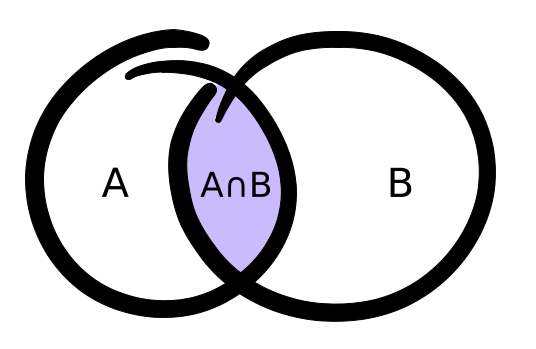
\includegraphics[scale=0.35]{FiguresBM/interseccion.png}
    		\caption[Representación de la intersección de dos conjuntos]{Representación de la intersección de dos conjuntos usando el diagrama de Venn. La zona oscurecida representa la intersección entre los conjuntos $A$ y $B$.}
	\end{figure}
\end{center}
Si dos conjuntos tienen intersección vacía se llaman \textit{conjuntos disjuntos}. Se escriben de la forma $A\cap B=\{\}$ o $A\cap B=\varnothing$.
\subsection{Unión de conjuntos}
La unión de dos conjuntos $A$ y $B$ contiene todos los elementos que pertenecen a $A$ y $B$. Esta operación es denotada por $A\cup B$ y se lee ``$A$ unido $B$'' o ``$A$ unión $B$''.\\
En términos de cuantificadores lógicos, la unión de conjuntos se representa de la siguiente manera:
\begin{equation}
A\cup B=\{x\in\mathcal{U}:x\in A\vee x\in B\}=\{x|x\in A\vee x\in B\}
\end{equation}
\begin{myexample}
Dado dos conjuntos finitos $A=\{a,b,c,d,e,f\}$ y $B=\{c,d,e,f,g,h\}$, determinar la unión $A\cup B$
\end{myexample}
\begin{equation*}
A\cup B=\{a,b,c,d,e,f,g,h\}
\end{equation*}
\begin{myexample}
Dado dos conjuntos finitos $A=\{1,1,1,1,1,1,2\}$ y $B=\{2,3\}$, determinar la unión $A\cup B$
\end{myexample}
\begin{equation*}
A\cup B=\{1,2,3\}
\end{equation*}

\begin{center}
	\begin{figure}[ht!]
	\centering
    		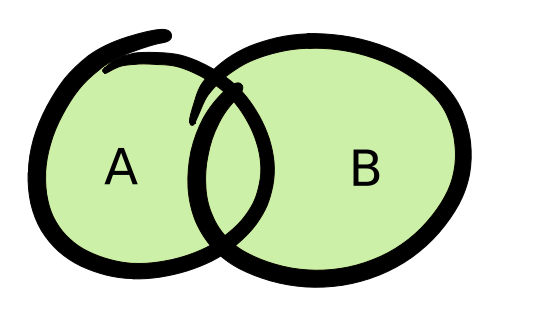
\includegraphics[scale=0.4]{FiguresBM/union.png}
    		\caption[Representación de la unión de dos conjuntos]{Representación de la unión de dos conjuntos usando el diagrama de Venn. La zona oscurecida muestra la unión entre el conjunto $A$ y $B$.}
	\end{figure}
\end{center}

\subsection{Diferencia simétrica de conjuntos}
La diferencia simétrica de dos conjuntos $A$ y $B$ es el conjunto que contiene la unión de ambos conjuntos, pero no considera la intersección de estos. La operación de diferencia simétrica se denota por $A\bigtriangleup B$ y en términos de cuantificadores se escribe de la siguiente manera:
\begin{equation*}
A\bigtriangleup B=\{x|x\in A\veebar B\}
\end{equation*}

\begin{center}
	\begin{figure}[ht!]
	\centering
    		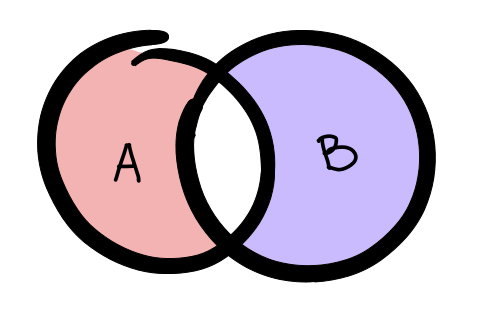
\includegraphics[scale=0.42]{FiguresBM/diferencias.png}
    		\caption[Representación de la diferencia simétrica entre el conjunto $A$ y $B$ ]{Representación de la diferencia simétrica entre el conjunto $A$ y $B$ usando el diagrama de Venn.}
	\end{figure}
\end{center}

\begin{myexample}
Sea dos conjuntos finitos $A=\{a,e,i,o,u\}$ y $B=\{a,b,c,d,e\}$. Calcular la diferencia simétrica entre los conjuntos $A$ y $B$.
\end{myexample}
\begin{eqnarray*}
A\bigtriangleup B =\{i,o,u,b,c,d\}
\end{eqnarray*}

\section{Propiedades de los conjuntos}
Con las operaciones vistas en (\ref{opc}) se ven importantes propiedades y ahora ocuparlas para reducir expresiones de dos o más conjuntos.

\subsection{Idempotencia}
La idempotencia es la propiedad de realizar una acción n-veces y aun así obtener el resultado como si se hubiera aplicado solo una vez.\\
\begin{eqnarray}
A\cup A&=& A\\
A\cap A&=& A
\end{eqnarray}

\begin{myexample}
Sea el conjunto finito $A=\{5,2,10\}$. Calcular $A\cup A$: 
\end{myexample}
\begin{eqnarray*}
A\cup A&=& \{5,2,10\}\cup\{5,2,10\} \nonumber\\
&=&\{5,2,10\} \\
&=&A
\end{eqnarray*}

%\begin{myexample}
%
%\end{myexample}
%\begin{eqnarray*}
%
%\end{eqnarray*}

\subsection{Conmutatividad}
La conmutatividad es la propiedad que tienen algunas operaciones en que el resultado de operar dos elementos no depende el orden en que se tomen estos mismos.\\
\begin{eqnarray}
A\cup B&=&B\cup A\\
A\cap B&=&B\cap A
\end{eqnarray}

\begin{myexample}
Sean los conjuntos finitos $A=\{Ibuprofeno,Naproxeno\}$ y \\ $B=\{ Aspirina,$ $Naproxeno,$ $Omeprazol \}$. Comprobar la propiedad conmutativa.
\end{myexample}
\begin{eqnarray*}
A\cap B&=& \{Ibuprofeno,Naproxeno\}\cap\{Aspirina,Naproxeno, Omeprazol \}\nonumber\\
&=& \{ Naproxeno\} \nonumber
\end{eqnarray*}
Análogamente
\begin{eqnarray*}
B\cap A&=&\{Aspirina, Naproxeno, Omeprazol \}\cap\{Ibuprofeno, Naproxeno\}\nonumber\\
&=& \{Naproxeno\}\nonumber\\
A\cap B &=& B\cap A \nonumber
\end{eqnarray*}

\subsection{Asociatividad}
La asociatividad es la propiedad de que el orden en que se ejecuten las operaciones no altera el resultado, siempre y cuando se mantenga intacto el orden de los elementos que se le aplica la operación (operandos).
\begin{eqnarray}
A\cup (B\cup C)&=&(A\cup B)\cup C\\
A\cap (B\cap C)&=&(A\cap B)\cap C
\end{eqnarray}
\subsection{Distributividad}
\begin{eqnarray}
A\cup (B\cap C)&=& (A\cup B)\cap(A\cup C)\label{distr0}\\
A\cap (B\cup C)&=& (A\cap B)\cup(A\cap C)
\end{eqnarray}

\begin{myexample}
Sean los conjuntos finitos $A=\{-5,-4,-3,-2,-1\}$, $B=\{-3,-2,-1,0,1,2,3\}$ y $C=\{-5,-2,-1,3,4\}$. Comprobar la propiedad distributiva
\end{myexample}
Primero se calcula el lado izquierdo de la ecuación (\ref{distr0}).
\begin{eqnarray}
A\cup (B\cap C) &=& \{-5,-4,-3,-2,-1\}\cup(\{-3,-2,-1,0,1,2,3\}\cap\{-5,-2,-1,3,4\}) \nonumber\\
&=& \{-5,-4,-3,-2,-1\}\cup\{-2,-1,3\}\nonumber\\
&=&\{-5,-4,-3,-2,-1,3\}\label{distr1}
\end{eqnarray}
ahora se desarrolla el lado derecho de la ecuación (\ref{distr0}).
\begin{eqnarray}
(A\cup B)\cap(A\cup C)&=&(\{-5,-4,-3,-2,-1,0,1,2,3\})\cap(\{-5,-4,-3,-2,-1,3,4\})\nonumber\\
&=&\{-5,-4,-3,-2,-1,3\}\label{distr2}
\end{eqnarray}
Como se puede ver, por las ecuaciones (\ref{distr1}) y (\ref{distr2}) se comprueba la propiedad distributiva de los conjuntos.

\subsection{Leyes de Morgan}
\begin{eqnarray}
(A\cup B)^{c}&=& A^{c}\cap B^{c}\\
(A\cap B)^{c}&=& A^{c}\cup B^{c}
\end{eqnarray}
\begin{myexample}
Demostrar mediante cuantificadores lógicos la expresión $(A\cap B)^{c}=A^{c}\cup B^{c}$
\end{myexample}

\begin{eqnarray}
x\in (A\cap B)^{c} &\Leftrightarrow & x\notin A\cap B \nonumber\\
&\Leftrightarrow & \sim ((x\in A)\wedge(x\in B))\nonumber\\
&\Leftrightarrow &\sim (x\in A)\vee\sim(x\in B)\nonumber\\
&\Leftrightarrow & x\in A^{c} \vee x\in B^{c}\nonumber\\
&\Leftrightarrow & x\in A^{c}\cup B^{c}\nonumber
\end{eqnarray}
Entonces se comprueba que $(A\cap B)^{c}=A^{c}\cup B^{c}$.


\section{Técnicas de conteo}
Para completar el conocimiento que se puede tener sobre un conjunto (o varios conjuntos) falta agregar las herramientas que nos permitan saber cuantos elementos tienen cada conjunto. Las técnicas de conteo solucionan esta problemática usando el concepto de cardinalidad (definido en \ref{cardinalidad}) y para dos casos, cuando los conjuntos no tienen intersección o si la tienen.
\subsection{Conteo en conjuntos disjuntos}
Como en este caso la intersección entre los conjuntos es vacía, la cardinalidad de la unión entre los conjuntos $A$ y $B$ está dada por:
\begin{equation}
|A\cup B|=|A|+|B| \label{conteo0}
\end{equation}
\begin{myexample}
Sea $A=\{1,2,3\}$ y $B=\{a,b,c\}$ dos conjuntos finitos y disjuntos. Mostrar la cardinalidad de la unión entre $A$ y $B$.
\end{myexample}
\begin{eqnarray*}
|A\cup B|=|A|+|B|=3+3=6
\end{eqnarray*}
Notar que $A\cup B=\{1,2,3,a,b,c\}$ y tiene cardinalidad 6. 
\begin{myexample}
En el examen único nacional de medicina (EUNACOM) del 2017\footnote{Informe final EUNACOM, enero 2018. Fuente: www.eunacom.cl} el área de Medicina interna tuvo $67$ preguntas, mientras que en pediatría fueron $29$. Si consideramos ambas áreas como conjuntos, ¿Cuál es la cardinalidad de la unión de ambos conjuntos? 
\end{myexample}
Identificaremos el conjunto de medicina interna como $MI$ y el de pediatría como $P$, ahora se aplica la ecuación (\ref{conteo0}) y resulta lo siguiente:
\begin{eqnarray}
|MI\cup P|=|MI|+|P|=67+29=96.
\end{eqnarray}

Además, mencionar que esto se puede expandir para $n$ conjuntos donde se debe sumar la cardinalidad de cada conjunto, ya que no hay intersección entre ellos.

\subsection{Conteo en conjuntos no disjuntos}
Para el caso en que si hay intersección entre dos conjuntos se sigue la misma lógica, pero se debe quitar la cardinalidad de la intersección para no cometer el error de contar dos veces algunos elementos.
\begin{equation}
|A\cup B|=|A|+|B|-|A\cap B|
\end{equation}
\begin{myexample}
Sea $A=\{1,2,3\}$ y $B=\{3,4,5\}$ dos conjuntos finitos y no disjuntos. Mostrar la cardinalidad de la unión entre estos dos conjuntos.
\end{myexample}
\begin{eqnarray}
|A\cup B|&=&|A|+|B|-|A\cap B|\nonumber\\
&=& 3+3-1=5\nonumber
\end{eqnarray}

\subsection{Conteo para la unión de tres conjuntos}
La ecuación para el caso de tres conjuntos se puede derivar de la ecuación para dos conjuntos no disjuntos.
\begin{eqnarray}
|A\cup B\cup C|&=&|A\cup (B\cup C)|\nonumber\\
&=&|A|+|B\cup C|-|A\cap (B\cup C)| \nonumber\\
&=&|A|+|B|+|C|-|B\cap C|-|A\cap (B\cup C)|\nonumber\\
&=&|A|+|B|+|C|-|B\cap C|-|(A\cap B)\cup(A\cap C)|\nonumber\\
&=&|A|+|B|+|C|-|B\cap C|-(|A\cap B|+|A\cap C|-|(A\cap B)\cap(A\cap C)|)\nonumber\\
&=&|A|+|B|+|C|-|B\cap C|-|A\cap B|-|A\cap C|+|(A\cap B)\cap(A\cap C)|\nonumber\\
&=&|A|+|B|+|C|-|B\cap C|-|A\cap B|-|A\cap C|+|A\cap B\cap C|
\label{uni3c}
\end{eqnarray}
La ecuación (\ref{uni3c}) muestra la ecuación para contar la unión de tres conjuntos no disjuntos.

Adicionalmente, desde el diagrama de Venn se puede definir las formulas para el número de elementos que solo se encuentran en un solo conjunto como solo en las intersecciones.\\

\begin{center}
\textbf{Número de elementos en un solo conjunto}\\
\end{center}


\noindent Los elementos que solo están en A:
\begin{eqnarray}
E_{A}=|A|-|A\cap B|-|A\cap C|+|A\cap B\cap C|
\end{eqnarray}
\noindent Los elementos que solo están en B:
\begin{eqnarray}
E_{B}=|B|-|A\cap B|-|B\cap C|+|A\cap B\cap C|
\end{eqnarray}
\noindent Los elementos que solo están en C:
\begin{eqnarray}
E_{C}=|C|-|A\cap C|-|B\cap C|+|A\cap B\cap C|
\end{eqnarray}

\begin{center}
\textbf{Número de elementos en la intersección de dos conjuntos, pero no en el tercero}\\
\end{center}

\noindent El número de elementos que están en $A\cap B$, pero no en C:\\
\begin{eqnarray}
E_{A\cap B}=|A\cap B|-|A\cap B\cap C|
\end{eqnarray}

\noindent El número de elementos que están en $A\cap C$, pero no en B:\\
\begin{eqnarray}
E_{A\cap C}=|A\cap C|-|A\cap B\cap C|
\end{eqnarray}

\noindent El número de elementos que están en $B\cap C$, pero no en A:\\
\begin{eqnarray}
E_{B\cap C}=|B\cap C|-|A\cap B\cap C|
\end{eqnarray}

\begin{center}
\textbf{Número de elementos en la unión de dos conjuntos, pero no en el tercero}\\
\end{center}

\noindent El número de elementos que está en $A$ o en $B$, pero no está en C:\\
\begin{eqnarray}
E_{A\cup B}=|A\cup B|-|A\cap B|-|B\cap C|+|A\cap B\cap C|
\end{eqnarray}

\noindent El número de elementos que está en $A$ o en $C$, pero no está en B:\\
\begin{eqnarray}
E_{A\cup C}=|A\cup C|-|A\cap B|-|B\cap C|+|A\cap B\cap C|
\end{eqnarray}

\noindent El número de elementos que está en $B$ o en $C$, pero no está en A:\\
\begin{eqnarray}
E_{B\cup C}=|B\cup C|-|A\cap B|-|A\cap C|+|A\cap B\cap C|
\end{eqnarray}

\begin{myexample}
Se encuestó a $100$ médicos sobre sus preferencias de especialidad y las respuestas arrojaron lo siguiente:
\end{myexample}
\begin{itemize}
	\item 32 Cirugía Pediátrica, $|CP|=32$.
	\item 20 Genética Clínica, $|GC|=20$.
	\item 45 Dermatología, $|D|=45$.
	\item 15 Cirugía pediátrica y Dermatología, $|CP\cap D|=15$.
	\item 7 Cirugía Pediátrica y Genética Clínica, $|CP\cap GC|=7$.
	\item 10 Genética Clínica y Dermatología, $|GC\cap D|=10$.
	\item 30 no prefieren ninguna de las tres especialidades.
\end{itemize}
\noindent a) Encontrar, el número de médicos que estudian las tres asignaturas.\\

Primero, notar que el número de médicos encuestados es el conjunto universo, entonces $\mathcal{U}=100$. Por lo que la unión de los tres conjuntos es:\\
\begin{eqnarray*}
|CP\cup GC\cup D|=100-30=70
\end{eqnarray*}
Segundo, de la ecuación (\ref{uni3c}) nos faltan dos términos, $|A\cup B\cup C|$ y $|A\cap B\cap C|$. Siendo el segundo el que se busca.

\begin{eqnarray*}
|CP\cup GC\cup D|&=&|CP|+|GC|+|D|-|CP\cap GC|-|CP\cap D|-|GC\cap D|+|CP\cap GC\cap D| \\
70&=&32+20+45-7-15-10+|CP\cap GC\cap D|\\
|CP\cap GC\cap D|&=&70-32-20-45+7+15+10\\
|CP\cap GC\cap D|&=&5\\
\end{eqnarray*}
Solo 5 médicos prefieren las tres especialidades.\\

\noindent  b) Encontrar el numero de médicos que prefieren una y solo una de las tres especialidades.\\

Se debe encontrar el número de médicos que prefiere una y solo una especialidad por separado.\\

\noindent Solo prefieren Cirugía Pediátrica:
\begin{eqnarray*}
|CP|-|CP\cap GC|-|CP\cap D|+|CP\cap GC\cap D| &=& 32-7-15+5=15\\
\end{eqnarray*}
Solo prefieren Genética Clínica:
\begin{eqnarray*}
|GC|-|GC\cap CP|-|GC\cap D|+|CP\cap GC\cap D| &=&20-7-10+5=8\\
\end{eqnarray*}
Dermatología :
\begin{eqnarray*}
|D|-|D\cap GC|-|D\cap CP|+|CP\cap GC\cap D| &=&45-10-15+5=25\\
\end{eqnarray*}
Finalmente el total de médicos que prefieren una y solo especialidad es: $15+8+25=48$ médicos.\\